\documentclass{article}
    \usepackage{caption}
    \usepackage{subcaption}
    \usepackage{mathtools}
    \usepackage{algorithm2e}
    
    \usepackage{enumerate}% section item
    \usepackage{amssymb}  % \varnothing
    \usepackage{booktabs} % insert table
    \usepackage{multirow} % table combine
    \usepackage{listings} % insert code
    \usepackage{appendix} % 
    \usepackage{amsmath}  % for mathfont
    \usepackage{unicode-math} % for mathfont
    \usepackage{fontspec} % set font
    \setmainfont{Times} % main font
    \newfontfamily\monaco{Monaco} % code font
    \usepackage{pythonhighlight} % python
   % \usepackage{hyperref}




    \usepackage[colorlinks=true]{hyperref} % the option is there to remove the square around links which is what I don't like.
    
    \usepackage{perpage} 
    \MakePerPage{footnote} % Reset the footnote counter perpage. may require to run latex twice.
    
    \usepackage[margin=2cm]{geometry} % This is here to fit more text into the page.
    
 %   \setcounter{secnumdepth}{1}  % This removes the numbering from the subsections.
                            % If you want the numbering of the subsection level just remove this line
    
    \title{\textsc{COMP7506 - CourseSchedule}}
    \author{	
                3035562502 - ZHANG Kai \\
                3035562100 - WANG Dezhao \\
                3035562069 - YAN Qiangyu }
    \date{}
    
    \setlength{\parindent}{0pt} % No indentation for paragraphs. Because that is just old.
    \setlength{\parskip}{\baselineskip} % Instead use vertical paragraph spacing.
    
    %\setmainfont{Helvetical} % Setting the main font here. But I like the default font alot so this is commented out.
    
    \begin{document}
    \maketitle
    
    
    \section{Background Research}

    \subsection{Category \& Function Synopsis}
    CourseSchedule is an eduactional Andriod application that aims to 
    make HKU students get their course schedule easier.
    
    In this App, students can get their course schedule
    once they logged in with right portal account, 
    and it's the mian function of this App.
    With this App, users can view their course with different colors.
    Meanwhile, this App also provides the function of GPA calculator,
    add the events to calendar, add notes, check the exam time, etc.

    \subsection{Market Analysis}
    There are some similar eduactional App in the market, 
    have different features and functions,
    but most of them only provide the course schedule of \textbf{mainland universities}.
    
    HKU as an international university has thousands of students 
    all over the world, and they all need to view the course information
    whenever they go to school. 
    Usually, students get the course information by visiting the HKU website.
    For CS postgraduate programme students, they need to view 
    the course information via CS intranet, which is more difficult for
    the App that posted in the App store to get.
    
    Based on thess fact and considering the inconvenience of 
    checking the course information of
    CS postgraduate programme students in HKU, 
    we designed this App, and we believe that
    this App will have a considerable market.
    With this App, students will be able to check their course schedule
    more easier, and their only need to log in this App only once,
    this is one of its conveniences.

    Besides, this App provides the function of checking the exam timetable,
    which transform the big exam timetable 
    which shows all the exam that faculty holds into 
    the specific exam timetable of usres themselves.
    And along with the timetable, it also comments with the notes
    given by the office, such as "bring the calculator", 
    "bring A4 paper sheet".
    Thus users do not need to check the informs one by one, 
    this is another of its conveniences.

    With these main features, students of CS postgraduate programme
    may have a motivation to download this App, and with the download,
    they will find this App have more useful functions like 
    GPA calculator, calendar adding and making notes.
    These functions will help users to schedule their time more easier
    and have benifits on their study, which are attractive for students.

    Even constrain this App's target users to 
    the student of CS postgraduate programme, 
    it will have a "big" market based on the consideration of
    the time cost in its developing.
    This App will have a considerable market because of 
    its own useful functions and the fact 
    that the market did not provides any similar Apps 
    that can applied out of mainland.

    Once we got more supports by other departments, 
    this App may be popular in the whole school of HKU.





    \subsection{Similar Apps}
    \subsubsection{QSC}
    \begin{center}
        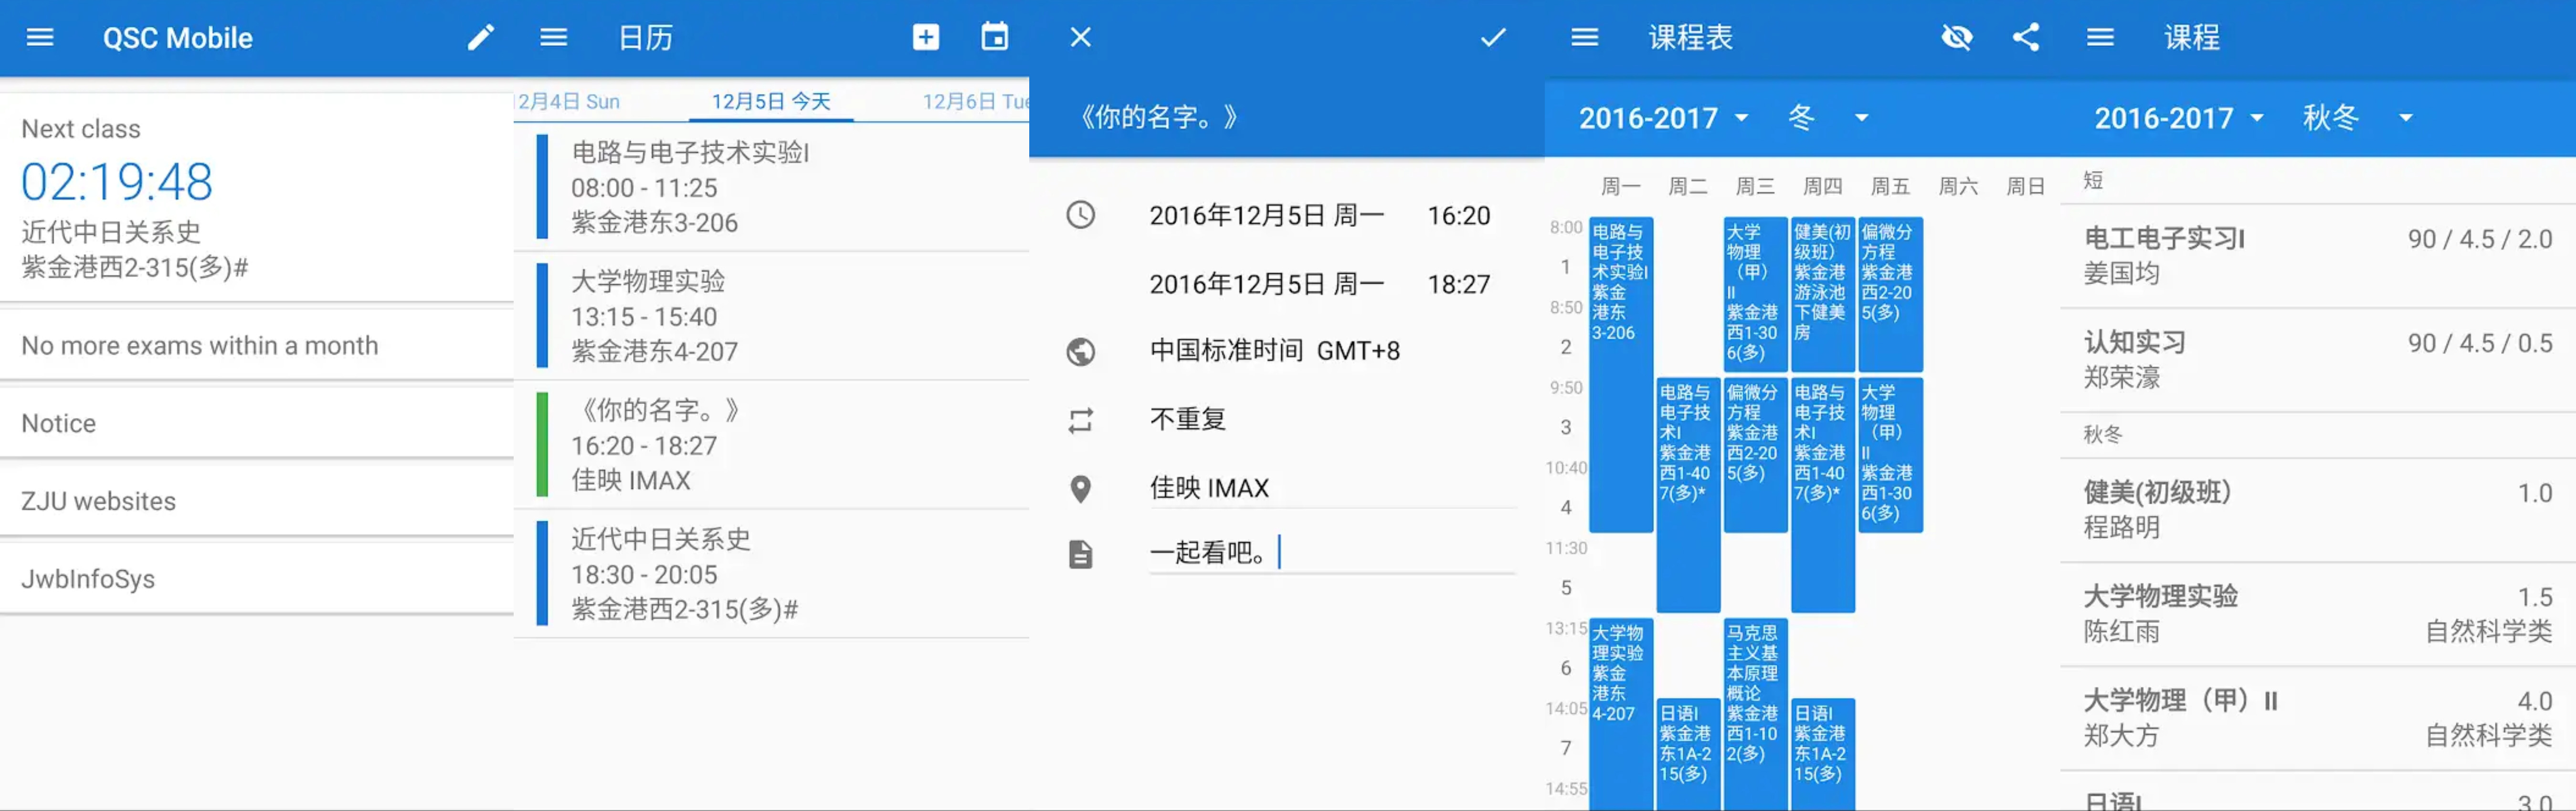
\includegraphics[width=6.9in]{QSC}
    \end{center}
    \begin{enumerate}[i)]

    \item Main Features

    - Show course schedule in days and weeks, with exam countdown.

    - Users can add the calendar to this App.

    - Review users' GPA.

    - Check the useful website.

    \item Short-Comings / Possible Improvements
    
    - Only provide the service for Zhejiang University.
    
    - All the course lookes similar.

    - Other web information are just copy to the App.

    \end{enumerate}
    

    \subsubsection{CourseGrid}
    \begin{center}
        
\includegraphics[width=6.5in]{CourseGrid}
    \end{center}
    \begin{enumerate}[i)]

    \item Main Features

    - Quick access to class schedules and 
    docking of more than 1,500 university educational systems.

    - A collection of practical tools, such as CET scores checking.
    
    - Combined with ZAKER News, providing quality reading content.
    
    - Provide a job plaza.

    \item Short-Comings / Possible Improvements
    
    - Too many useless information.

    - Cannot add other schedules or make notes.

    - Cannot provide the GPA review.

    - Cannot access the course schedule of HKU.

    \end{enumerate}


    \subsubsection{SuperCurriculum}
    \begin{center}
        
\includegraphics[width=6.5in]{SuperCurriculum}
    \end{center}
    \begin{enumerate}[i)]

    \item Main Features

    - Quick access to class schedules.

    - A collection of practical tools, such as CET scores checking.
    
    - Provide a alumni platform.

    \item Short-Comings / Possible Improvements
    
    - Too many useless information, like a social tool.

    - Cannot add other schedules or make notes.

    - Cannot access the course schedule of HKU.

    \end{enumerate}




    \section{App Features}

    \begin{enumerate}[a)]
    \item Succinct UI Desgin
    
    We make the Ui succinct by only show 
    
    \item Colorful View
    
    
    
    \end{enumerate}
    
 


    
    \section{Contributions}

    \begin{table}[h]
        \centering
        \begin{tabular}{|c|l|}
            \hline
            \multirow{7}{*}{ZHANG Kai} &  Main activity with layout/main.xml\\
            \cline{2-2}
            &Switch fragment functions \\
            \cline{2-2}
            &Fragment of homepage, corresponding layout xml file \\
            \cline{2-2}
            &Toolbar function and xml, bind toggle icon with drawer listener \\
            \cline{2-2}
            & Custom HolderView implements Holder, 
            implement automatic scrolling of pictures with\\
            & ConvenientBann\\
            \cline{2-2}
            &Complete the draft documentation, and Readme.md \\
            \hline
            \multirow{7}{*}{WANG Dezhao} &  
            Fragment of basic info (fees, overview, schedule), 
            corresponding layout xml files\\
            \cline{2-2}
            & Fragment of about (faculty, about HKU), 
            corresponding layout xml files \\
            \cline{2-2}
            & Custom ExpandableListAdapter and MenuModel item, 
            with list\_group\_child.xml/ \\
            & list\_group\_header.xml,
             generate custom drawer controls \\
            \cline{2-2}
            & View pager function, custom pager adapter \\
            \cline{2-2}
            & Page view layout files including Programme Overview, 
            Stream of Study, Selection of Courses, \\
            & Dissertations \\
            \hline
            \multirow{7}{*}{YAN Qiangyu} &  
            Fragment of news \& events, corresponding layout xml files\\
            \cline{2-2}
            & Custom loading view \\
            \cline{2-2}
            & Custom card view of news and card view of events \\
            \cline{2-2}
            & Multi-threaded operation when using Jsoup 
            to scratch message from URL and parse HTML \\
            \cline{2-2}
            & Update UI by using UIThread \\
            \cline{2-2}
            & Make the video \\
            \cline{2-2}
            & Review and complete the final documentation \\
            \hline
        \end{tabular}
    \end{table}

    \end{document}